\beginsong{Trinklied vom Abgang}[
    txt={Theodor Kramer}, 
    mel={Erich Schmeckenbecher}, 
    jahr={1943}, 
    bo={276}, 
    siru={206}, 
    index={Schon wird uns oft},
]

\beginverse
\endverse
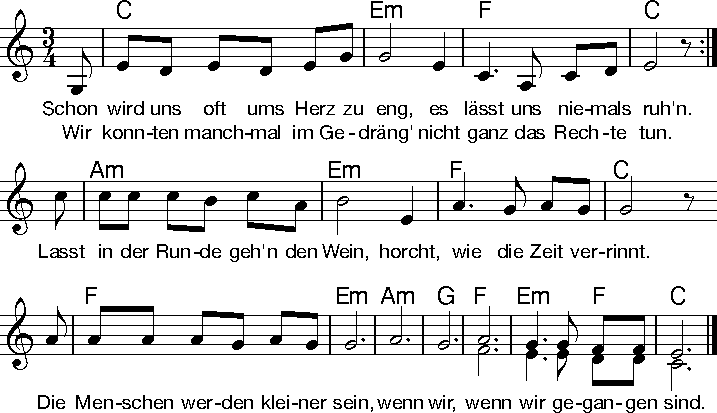
\includegraphics[draft=false, width=1\textwidth]{Noten/Lied085.pdf}	

\beginverse
Uns \[C]wäre eingereiht, be\[Em]haust und \[F]vorbetreuet nicht \[C]wohl, wir
konnten doch in uns'rer \[Em]Faust ver\[F]einen Pol und \[C]Pol. Lasst
\[Am]in der Runde geh'n den \[Em]Wein, horcht, \[F]wie die Zeit ver\[C]rinnt, die
\[F]Menschen werden schwächer \[Em]sein, \[Am]wenn \[G]wir, \[F]wenn \[Em]wir ge\[F]gangen \[C]sind.
\endverse

\beginverse
Ob ^altes Maß, ob neues ^Maß, wir ^müssen bald Ver^geh'n, was
schadet's, bleibt nur dies und ^das von ^uns als Zeichen ^stehn. Lasst
^in der Runde geh'n den ^Wein, horcht, ^wie die Zeit ver^rinnt, die
^Menschen werden freier ^sein, ^wenn ^wir, ^wenn ^wir ge^gangen ^sind.
\endverse

\endsong
